\documentclass{article}
\usepackage{graphicx}
\graphicspath{{figures/}}
\usepackage{subfigure}
\usepackage{amsmath}
\usepackage{listings}

\usepackage{color} %red, green, blue, yellow, cyan, magenta, black, white
\definecolor{mygreen}{RGB}{28,172,0} % color values Red, Green, Blue
\definecolor{mylilas}{RGB}{170,55,241}

\title{Sections and Chapters}
\author{Gubert Farnsworth}
\date{ ENME 625: Multi-Displinary Optimization \\ 5/12/2017}
 
\begin{document}
 
\maketitle

\newpage
 
\tableofcontents
 
\newpage 
 
\section{Introduction}
 
This is the first section.
 

\section{Unconstrained MOGA Problems}
We used this textbook \cite{deb2001multi}

\subsection{ZDT1} 
The first test problem, denoted as ZDT1 in (insert reference) is shown below. 


\begin{align*}
\textrm{Minimize} ~~~~~ f_1(\textbf{x}) &= x_1 \\
\textrm{Minimize} ~~~~~ f_2(\textbf{x}) &= g(x)*h(x) \\
\textrm{where} ~~~~~~~~~~ g(x) &= 1+\frac{9}{(n-1)}\sum_{i=2}^{n}x_i \\
~~~~~~~~~~ h(x) &= 1- \sqrt{\frac{f_1(x)}{g(x)}} \\
~~~~~~~~~~ n &= 30 \\
0 &\leq  \textbf{x}  \leq 1 \\
\end{align*}

The true Pareto frontier for this problem occurs when $x_i = 0$ for i = 2,...,30. Figure~\ref{fig:ZDT1} shows a sample result from both MATLABs built in MOGA and the MOGA developed in this project. The quality metrics chosen to evaluate this problem are Coverage Difference (CD)and Pareto Spread (OS). Ten runs for each algorithm were performed and the mean and standard deviation of each metric are tabulated in Table~\ref{tab:ZDT1}.
\begin{figure}[h]
  \caption{Example Pareto Results for ZDT1}
  \centering
  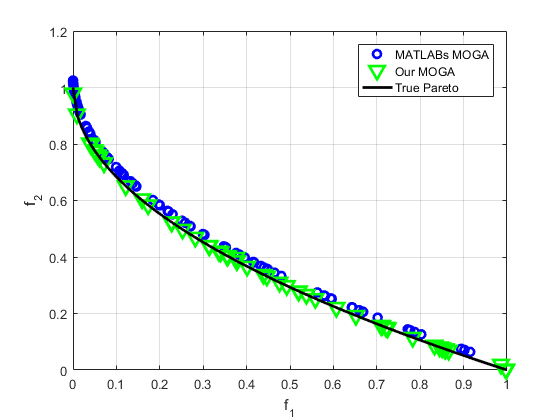
\includegraphics[width=0.85\textwidth]{ZDT1_pareto_final.png}  
  \label{fig:ZDT1}
\end{figure}

\begin{table}[h]
\caption{Quality Metrics for ZDT1} 
\centering 
\begin{tabular}{|c|c|c|} 
\hline\hline  
Metric & MATLABs MOGA & Our MOGA \\ \hline
CD & 0.3874 (0.0164) &  0.3582 (0.0040) \\ \hline
OS & 0.9605 (0.1088) & 0.9283 (0.0928) \\ \hline
\end{tabular}
\label{tab:ZDT1} 
\end{table}
From these metrics, there is certainly a trade-off between MATLABs MOGA and the MOGA developed in this project. The coverage difference of the new MOGA is better in this problem whereas the Pareto spread is improved when using MATLABs MOGA. 

\subsection{ZDT2} 
The second test problem, denoted as ZDT2 in (insert reference) is shown below. 


\begin{align*}
\textrm{Minimize} ~~~~~ f_1(\textbf{x}) &= x_1 \\
\textrm{Minimize} ~~~~~ f_2(\textbf{x}) &= g(x)*h(x) \\
\textrm{where} ~~~~~~~~~~ g(x) &= 1+\frac{9}{(n-1)}\sum_{i=2}^{n}x_i \\
~~~~~~~~~~ h(x) &= 1- \frac{f_1(x)}{g(x)}^2 \\
~~~~~~~~~~ n &= 30 \\
0 &\leq  \textbf{x}  \leq 1 \\
\end{align*}

The true Pareto frontier for this problem, similar to ZDT1, occurs when $x_i$ = 0 for i = 2,...,30. Figure~\ref{fig:ZDT2} shows a sample result from both MATLABs built in MOGA and the MOGA developed in this project. Table~\ref{tab:ZDT2} summarizes the mean quality metrics for each algorithm for ten runs.
\begin{figure}[h!]
  \caption{Example Pareto Results for ZDT2}
  \centering
  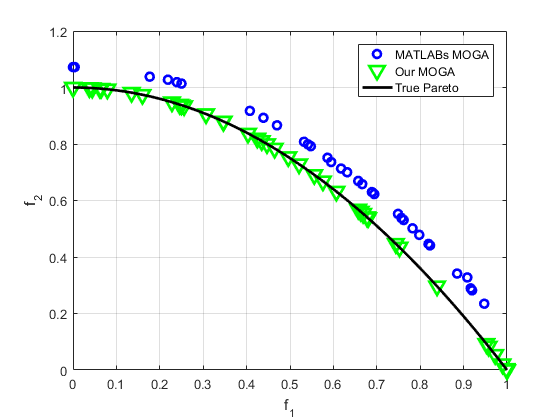
\includegraphics[width=0.85\textwidth]{ZDT2_pareto_final.png}  
  \label{fig:ZDT2}
\end{figure}

\begin{table}[h]
\caption{Quality Metrics for ZDT2} 
\centering 
\begin{tabular}{|c|c|c|} 
\hline\hline  
Metric & MATLABs MOGA & Our MOGA \\ \hline
CD & 0.7832  (0.0821) & 0.6971  (0.0094) \\ \hline
OS &  0.8781 (0.0946) & 1.0086 (0.0278)  \\ \hline
\end{tabular}
\label{tab:ZDT2} 
\end{table}

\subsection{ZDT3} 
The third test problem, denoted as ZDT3 in (insert reference) is shown below. 


\begin{align*}
\textrm{Minimize} ~~~~~ f_1(\textbf{x}) &= x_1 \\
\textrm{Minimize} ~~~~~ f_2(\textbf{x}) &= g(x)*h(x) \\
\textrm{where} ~~~~~~~~~~ g(x) &= 1+\frac{9}{(n-1)}\sum_{i=2}^{n}x_i \\
~~~~~~~~~~ h(x) &= 1- \sqrt{\frac{f_1(x)}{g(x)}}- \frac{f_1(x)}{g(x)}\sin(10\pi f_1) \\
~~~~~~~~~~ n &= 30 \\
0 &\leq  \textbf{x}  \leq 1 \\
\end{align*}

The true Pareto frontier for this problem again occurs when $x_i$ = 0 for i = 2,...,30. Figure~\ref{fig:ZDT3} shows a sample result from both MATLABs built in MOGA and the MOGA developed in this project. Table~\ref{tab:ZDT3} summarizes the mean quality metrics for each algorithm for ten runs.

\begin{figure}[h]
  \caption{Example Pareto Results for ZDT3}
  \centering
  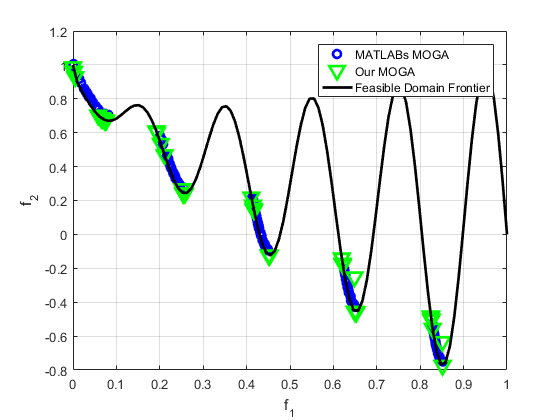
\includegraphics[width=0.85\textwidth]{ZDT3_pareto_final.png}  
  \label{fig:ZDT3}
\end{figure}

\begin{table}[h]
\caption{Quality Metrics for ZDT3} 
\centering 
\begin{tabular}{|c|c|c|} 
\hline\hline  
Metric & MATLABs MOGA & Our MOGA \\ \hline
CD & 0.7407 (0.0050) & 0.7554 (0.0031) \\ \hline
OS & 0.8565 (0.0098) & 0.8489 (0.0180) \\ \hline
\end{tabular}
\label{tab:ZDT3} 
\end{table}

Overall, MATLABs MOGA outperforms the MOGA developed in this project in both coverage difference and Pareto spread. A paired t-test shows that the difference in the means for coverage difference is statistically significant (p<0.05), while the difference is not statistically significant in Pareto Spread (p=0.21). 

\subsection{OSY} 
This test problem, denoted as OSY in (insert reference) is shown below. 


\begin{align*}
\textrm{Minimize} ~~~~~ f_1(\textbf{x}) &= -(25(x_1-2)^2+(x_2-2)^2+(x_3-1)^2+(x_4-4)^2+(x_5-1)^2) \\
\textrm{Minimize} ~~~~~ f_2(\textbf{x}) &= \sum_{i=1}^{6}x_i^2 \\
\textrm{Subject to} ~~~~ g_1(x) &= 1-\frac{x_1+x_2}{2} \leq 0 \\
g_2(x) &= \frac{x_1+x_2}{6}-1 \leq 0 \\
g_3(x) &= \frac{x_2-x_1}{2}-1 \leq 0 \\
g_4(x) &= \frac{x_1-3x_2}{2}-1 \leq 0 \\
g_5(x) &= \frac{(x_3-3)^2+x_4}{4}-1 \leq 0 \\
g_6(x) &= 1-\frac{(x_5-3)^2+x_6}{4} \leq 0 \\
0 &\leq  x_1,x_2,x_6  \leq 10 \\
1 &\leq  x_3,x_5  \leq 5 \\
0 &\leq  x_4  \leq 6 \\
\end{align*}

The true Pareto frontier for this problem again occurs when $x_i$ = 0 for i = 2,...,30. Figure~\ref{fig:OSY} shows a sample result from both MATLABs built in MOGA and the MOGA developed in this project. Table~\ref{tab:OSY} summarizes the mean quality metrics for each algorithm for ten runs.
%\begin{figure}[h]
%  \caption{Example Pareto Results for OSY}
%  \centering
%  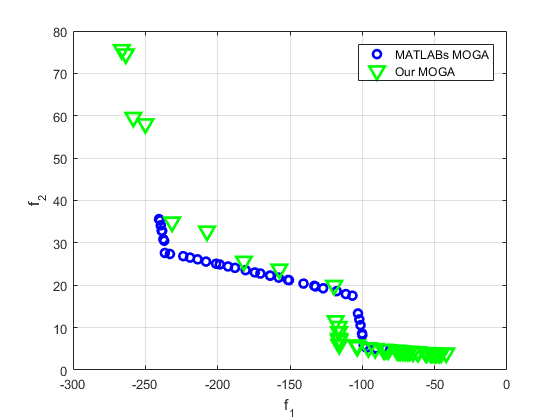
\includegraphics[width=0.85\textwidth]{OSY_pareto_final.png}  
%  \label{fig:OSY}
%\end{figure}

\begin{table}[h]
\caption{Quality Metrics for OSY} 
\centering 
\begin{tabular}{|c|c|c|} 
\hline\hline  
Metric & MATLABs MOGA & Our MOGA \\ \hline
CD &  &   \\ \hline
OS &  &  \\ \hline
\end{tabular}
\label{tab:OSY} 
\end{table}



\section{Constrained MOGA Problems}
This is a reference to Azarms constraint paper \cite{kurpati2002constraint}. %This is how references are read from the references.bib file.
 
\subsection{TNK} 
This test problem, denoted as TNK in (insert reference) is shown below with the true Pareto frontier shown in Figure~\ref{fig:TNK_true}.


\begin{align*}
\textrm{Minimize} ~~~~~ f_1(\textbf{x}) &= x_1 \\
\textrm{Minimize} ~~~~~ f_2(\textbf{x}) &= x_2 \\
\textrm{Subject to} ~~~~ g_1(x) &= -x_1^2-x_2^2+1+0.1\cos(16\arctan(\frac{x_1}{x_2})) \leq 0 \\
g_2(x) &= (x_1 - 0.5)^2 + (x_2 - 0.5)^2 -0.5 \leq 0 \\
0 &\leq  x_1,x_2 \leq \pi \\
\end{align*}
\begin{figure}[h]
  \caption{True Pareto Frontier for TNK}
  \centering
  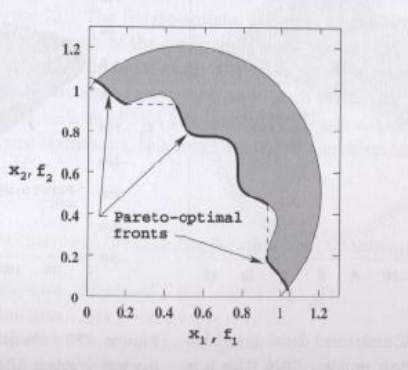
\includegraphics[width=0.85\textwidth]{TNK_pareto_true.png}  
  \label{fig:TNK_true}
\end{figure}


Figure~\ref{fig:TNK} shows a sample result from both MATLABs built in MOGA and the MOGA developed in this project. Table~\ref{tab:TNK} summarizes the mean quality metrics for each algorithm for ten runs.
\begin{figure}[h]
  \caption{Example Pareto Results for TNK}
  \centering
  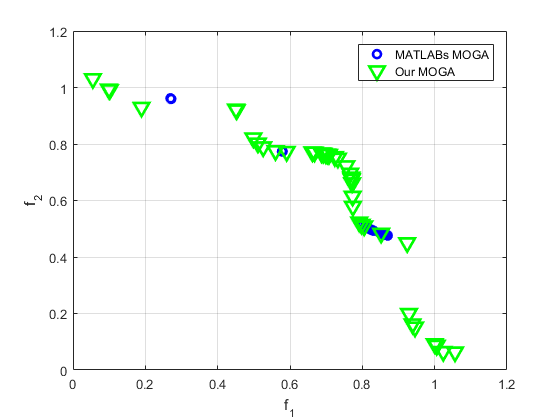
\includegraphics[width=0.85\textwidth]{TNK_pareto_final.png}  
  \label{fig:TNK}
\end{figure}

\begin{table}[h]
\caption{Quality Metrics for TNK} 
\centering 
\begin{tabular}{|c|c|c|} 
\hline\hline  
Metric & MATLABs MOGA & Our MOGA \\ \hline
CD &  0.8581 (0.0480) & 0.7792 (0.0036) \\ \hline
OS & 0.4177 (0.3216) & 0.9763 (0.0178)\\ \hline
\end{tabular}
\label{tab:TNK} 
\end{table}
 
Comparing the estimated Pareto frontiers to the true Pareto frontier, is is clear that our MOGA outperforms MATLAB's MOGA. The Pareto spread in our MOGA is significantly higher however the coverage difference is higher in MATLABs MOGA (p<0.05).

\subsection{CTP} 
This test problem, denoted as CTP in (insert reference) is shown below and the true Pareto frontier is shown in Figure~\ref{fig:CTP_true}. 


\begin{align*}
\textrm{Minimize} ~~~~~ f_1(\textbf{x}) &= x_1 \\
\textrm{Minimize} ~~~~~ f_2(\textbf{x}) &= g(x)(1-\sqrt{\frac{f_1(x)}{g(x)}} \\
\textrm{Subject to} ~~~~ g_1(x) &= a|\sin(b\pi(\sin(\theta)(f_2(x)-e)+\cos(\theta)f_1(x))^c)|^d \\
&- \cos(\theta)(f_2(x)-e)-\sin(\theta)f_1(x) \leq 0 \\
\textrm{where} ~~~~~~~~~~ \theta &= -0.2\pi, a = 0.2, b=10, c=1, d=6, e = 1 \\
g(x) &= |1+(\sum_{i=2}^{10}x_i)^{0.25}| \\
0 &\leq  x_1  \leq 1 \\
-5 &\leq  x_i  \leq 5, i = 2,...,10 \\
\end{align*}
\begin{figure}[h]
  \caption{True Pareto Frontier for CTP}
  \centering
  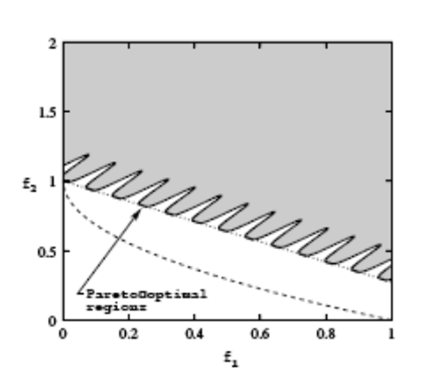
\includegraphics[width=0.85\textwidth]{CTP_pareto_true.png}  
  \label{fig:CTP_true}
\end{figure}

Figure~\ref{fig:CTP} shows a sample result from both MATLABs built in MOGA and the MOGA developed in this project. Table~\ref{tab:CTP} summarizes the mean quality metrics for each algorithm for ten runs.
\begin{figure}[h]
  \caption{Example Pareto Results for CTP}
  \centering
  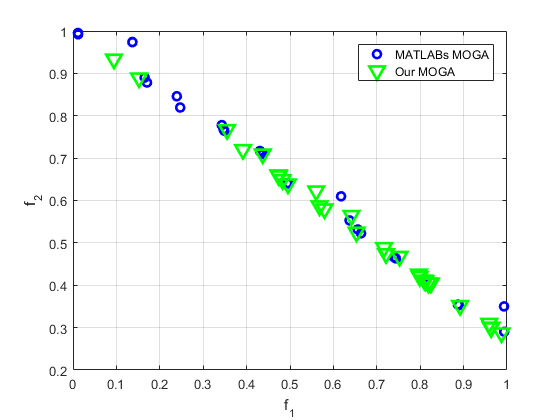
\includegraphics[width=0.85\textwidth]{CTP_pareto_final.png}  
  \label{fig:CTP}
\end{figure}

\begin{table}[h]
\caption{Quality Metrics for CTP} 
\centering 
\begin{tabular}{|c|c|c|} 
\hline\hline  
Metric & MATLABs MOGA & Our MOGA \\ \hline
CD & 0.6802 (0.0067) &  0.6802 (0.0092) \\ \hline
OS & 0.7901 (0.0734) & 0.5959 (0.1324) \\ \hline
\end{tabular}
\label{tab:CTP} 
\end{table} 
 
The mean values for coverage difference are exactly the same for both algorithms. In fact a paired t-test also shows the means are not statistically difference(p>0.05). For Pareto spread, MATLAB's MOGA performs the highest.
 
 
 \newpage
\vspace{-0.1in}
\bibliographystyle{IEEEtran}
\bibliography{references.bib}
 
 

\section{Appendix}

%Matlab codes starts here
 

\lstset{language=Matlab,%
    %basicstyle=\color{red},
    breaklines=true,%
    morekeywords={matlab2tikz},
    keywordstyle=\color{blue},%
    morekeywords=[2]{1}, keywordstyle=[2]{\color{black}},
    identifierstyle=\color{black},%
    stringstyle=\color{mylilas},
    commentstyle=\color{mygreen},%
    showstringspaces=false,%without this there will be a symbol in the places where there is a space
    numbers=left,%
    numberstyle={\tiny \color{black}},% size of the numbers
    numbersep=8pt, % this defines how far the numbers are from the text
    emph=[1]{for,end,break},emphstyle=[1]\color{red}, %some words to emphasise
    %emph=[2]{word1,word2}, emphstyle=[2]{style},    
}


\section*{Matlab Code}

\lstinputlisting{MasterCode.m}
\lstinputlisting{fitFCN5.m}


\end{document}
